%%
%% This is file `sample-sigplan.tex',
%% generated with the docstrip utility.
%%
%% The original source files were:
%%
%% samples.dtx  (with options: `sigplan')
%% 
%% IMPORTANT NOTICE:
%% 
%% For the copyright see the source file.
%% 
%% Any modified versions of this file must be renamed
%% with new filenames distinct from sample-sigplan.tex.
%% 
%% For distribution of the original source see the terms
%% for copying and modification in the file samples.dtx.
%% 
%% This generated file may be distributed as long as the
%% original source files, as listed above, are part of the
%% same distribution. (The sources need not necessarily be
%% in the same archive or directory.)
%%
%% The first command in your LaTeX source must be the \documentclass command.
\documentclass[sigplan,screen,nonacm]{acmart}
\usepackage{color}
\usepackage{algorithm,algpseudocode}
\usepackage[
    type={CC},
    modifier={by-nc-sa},
    version={4.0},
]{doclicense}
%% NOTE that a single column version is required for 
%% submission and peer review. This can be done by changing
%% the \doucmentclass[...]{acmart} in this template to 
%% \documentclass[manuscript,screen,review]{acmart}
%% 
%% To ensure 100% compatibility, please check the white list of
%% approved LaTeX packages to be used with the Master Article Template at
%% https://www.acm.org/publications/taps/whitelist-of-latex-packages 
%% before creating your document. The white list page provides 
%% information on how to submit additional LaTeX packages for 
%% review and adoption.
%% Fonts used in the template cannot be substituted; margin 
%% adjustments are not allowed.
%%
%% \BibTeX command to typeset BibTeX logo in the docs
\AtBeginDocument{%
  \providecommand\BibTeX{{%
    \normalfont B\kern-0.5em{\scshape i\kern-0.25em b}\kern-0.8em\TeX}}}


%%
%% end of the preamble, start of the body of the document source.
\begin{document}

%%
%% The "title" command has an optional parameter,
%% allowing the author to define a "short title" to be used in page headers.
\title{Multipath TCP, and New Packet Scheduling Method}

%%
%% The "author" command and its associated commands are used to define
%% the authors and their affiliations.
%% Of note is the shared affiliation of the first two authors, and the
%% "authornote" and "authornotemark" commands
%% used to denote shared contribution to the research.
\author{Cole N. Maxwell}
\email{maxwe206@morris.umn.edu}
\affiliation{%
  \institution{Division of Science and Mathematics 
	\\
        University of Minnesota, Morris
	}
  \city{Morris}
  \state{Minnesota}
  \country{USA}
  \postcode{56267}
}
\begin{abstract}
Today many devices contain hardware to transmit data across the internet via cellular, WiFi, and wired connections. Many of these devices communicate by using a protocol known as Transmission Control Protocol (TCP).  TCP was developed when network resources were expensive, and it was rare for a typical network-aware device to have more than one connection to a network.  An extension to TCP known as Multipath TCP (MPTCP) was developed to leverage the multiple network connections to which devices now have access. While the MPTCP extension has been successful in its goal of using multiple network connections to send data simultaneously, MPTCP presents new challenges. Scheduling data to be sent across multiple network connections with varying network conditions can result in data arriving out of order, adding increased system overhead and network latency. This paper presents the challenges of MPTCP packet scheduling and summarizes a proposed solution that has been found to increase performance over existing MPTCP scheduling methods.
\end{abstract}
\doclicenseThis
\maketitle
\section{Introduction}
\label{sec:introduction}
Multipath transmission control protocol (MPTCP) is a network protocol that leverages 
the use of any network connections a device may have, for example, the cellular and WiFi connection of a smartphone, to deliver more failure-tolerant connections. Efficient scheduling of how data moves across all the connections a device has is challenging. Increasing MPTCP's network performance with new data scheduling methods is an active area of research. Section \ref{sec:background} provides the necessary background on basic computer networking, Transmission Control Protocol (TCP), the motivation for the MPTCP extension to TCP, and an overview of how MPTCP utilizes multiple network connections when facilitating communication between a client and server. Network metrics used to evaluate network performance are described in Section \ref{sec:metrics}. Section \ref{sec:method} provides an explanation of a proposed MPTCP scheduling method for heterogeneous wireless networks. The network simulations used to measure performance results of the proposed scheduling method are explained in Section \ref{sec:results}. The newly proposed MPTCP scheduling method was found to have an increase in overall network performance compared to other existing MPTCP scheduling methods.
\section{Background}
\label{sec:background}
The Internet Protocol (IP) is composed of a set of standards and techniques that underlay the exchange of information between two devices that are connected to the internet. Every device, or \emph{host}, connected to the internet is assigned an IP address, which is analogous to the traditional mailing address used by the Post Office. IP takes data provided by a host and divides that data into smaller pieces of information called \emph{packets}. IP attaches additional information to the start and end of each data packet, referred to as the header and footer of a packet. IP works similarly to placing a letter into an envelope, where the letter represents some piece of data, and a packet represents an envelope. The source and destination address are contained in the packet header much like the return and delivery address of an envelope. IP is only concerned with the movement of packets and does not handle packet ordering or error checking. To ensure data integrity additional data transport protocols are built on top of IP, the most common of which is TCP.
\subsection{Transmission Control Protocol}
\label{sec:tcp}
TCP is responsible for providing reliable data transmission that is error-checked upon delivery and presents that data to an application in the correct order. To provide this reliability, TCP requires two hosts to establish a connection before any data transmission can take place between them. The host that is attempting to access a resource from another host is called a \emph{client}. The host that is providing the resource to other hosts is called a \emph{server}. In order to establish a reliable connection to exchange a resource the client and server must perform a TCP three-way handshake. The steps for creating a connection are as follows and are also illustrated in Fig. \ref{fig:handshake}:
\begin{enumerate}
  \item The client sends a synchronize (SYN) informing the server that the client wants to start communication.
  \item The server responds to the client's request with an acknowledgment (ACK) of the client's request to start communication. Along with the ACK the server also sends a SYN informing the client that the server also seeks to start communication.
  \item The client sends a final ACK of the server’s request to start communication back to the server and a reliable connection with which the client and server can transfer data is established.
\end{enumerate}

\begin{figure}
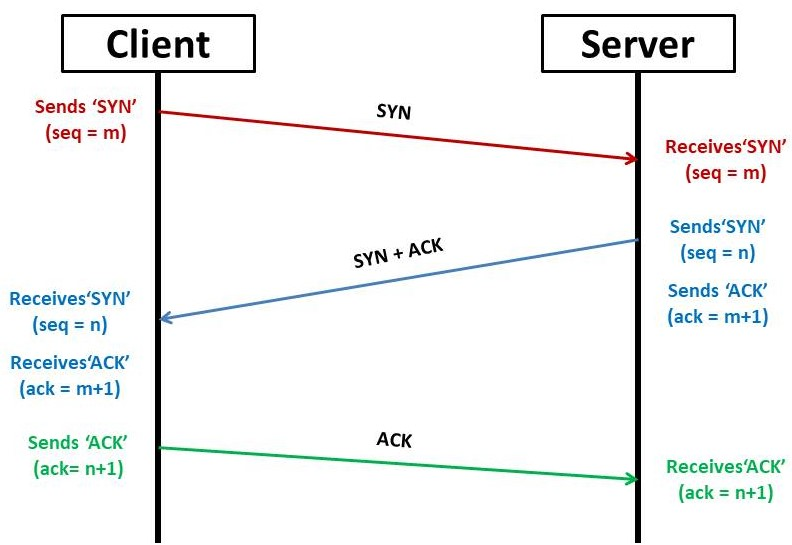
\includegraphics[width=2in]{mptcp_paper/assets/tcp-3-way-handshake.jpg}
\caption{An illustration of the TCP three-way handshake}
\label{fig:handshake}
\end{figure}

After a TCP connection is established, both the client and server can act as a sender and receiver of data in the connection. During the TCP handshake, several other options can be exchanged between the client and server regarding the parameters of the connection. The most important exchange in the three-way handshake are sequence and acknowledgment numbers which are used to detect missing or misordered data \cite{Stevens:2011}. When a host initiates a TCP session, its initial sequence number is effectively a random 32-bit number (between 0 and 4,294,967,295, inclusive). Here the initial sequence number will be discussed in relative terms, meaning that each side of a TCP session starts out with a relative sequence number of zero. Likewise, the acknowledgment number is also zero, as there is not yet a complementary side of the conversation to acknowledge. First, the client sends a SYN with a relative sequence number of zero. The server responds to the client with a sequence number of zero, as this is the first packet in this TCP session, and an acknowledgment number of 1 to indicate the receipt of the client's SYN. Notice that the acknowledgment number has been increased by 1 even though no data has yet been sent by the client. This is because the presence of the SYN is a received packet, which triggers an increase of 1 in the sequence. Next, the client ACK responds to the server's sequence number of zero with an acknowledgment number of 1. The client includes its own sequence number of 1, which has been incremented from zero because of the SYN. At this point, the sequence number for both hosts is 1. This initial increment of 1 on both hosts' sequence numbers occurs during the three-way handshake of all TCP sessions. Figure \ref{fig:handshake} also shows this process using absolute numbers rather than relative ones.

Now the first exchange of a data payload can take place. For example, the client might send a request for a resource to the server. Suppose the request for that resource required 100 bytes in total. Assuming the complete request is received by the server, the server's acknowledgment number will be increased by 100-- the ACK number is now 101. The server then responds with the resource requested by the client. The server's sequence number is still 1 since none of the server's packets (prior to this one) have carried a payload. Continuing our example, suppose that the resource being sent is 1500 bytes in total. Recall that the sequence number of the client has been increased to 101 because of the last packet the client sent. Upon receiving the 1500 bytes from the server, the client increases its acknowledgment number from 1 to 1501. As data continues to be exchanged between the client and server this process repeats. In the event that data goes missing, the receiver’s acknowledgment number will not be incremented by the full amount of the sender's sequence number. In this case, TCP can re-transmit the data until all of the data is successfully transferred to the receiver. 


While TCP provides reliable data transport, it was originally designed in the early 1970s. During this era, it was extremely uncommon for devices with network interfaces to have multiple mechanisms to deliver packets across a network. In today’s modern networks it is common for devices like smartphones to have cellular and WiFi connections simultaneously. The original TCP design does not allow devices to leverage multiple connections, called \emph{subflows}, because the connection is bound to the IP addresses of each party's network interface. \cite{MPTCPoverview:2012} Consider the case where a smartphone user is connected to a streaming music service via a WiFi connection. The TCP connection is bound to the IP address assigned to the WiFi interface of the smartphone. If the smartphone is moved from the home to a vehicle, losing WiFi connectivity, the connection will be interrupted. In order to continue the music stream, a new TCP connection must be established using the smartphone’s cellular network connection which is assigned a different IP address. This can result in service interruptions that pause the streaming music while establishing the new TCP connection. Network overhead is also increased when TCP connections need to be reestablished, putting an added burden on service providers.

\subsection{The MPTCP Extension}
\label{sec:mptcp}

To effectively use multiple network connections, the Internet Engineering Task Force (IETF) formally proposed the Multipath TCP extension of TCP in request for comment (RFC) 6824 in January of 2013. The standard was revised in 2020 in RFC 8684. Along with the specification, the RFC details two key features of MPTCP; it is compatible with the existing TCP standard, and MPTCP can operate over the same Internet infrastructure as TCP \cite{MPTCPoverview:2012}. MPTCP establishes a connection using the same three-way handshake described in section \ref{sec:tcp}. However, there are additional options exchanged:
\begin{enumerate}
  \item The client sends a SYN with the MP\_CAPABLE option which indicates the client is capable of using MPTCP. The option contains a token generated by the client, which will be used to identify the MPTCP session.
  \item The server responds with SYN-ACK which contains the MP\_CAPABLE option indicating the server is also capable of MPTCP and returns a session token generated by the server.
  \item The client sends an ACK and the first subflow is established. Data can now be transmitted on the first subflow.
\end{enumerate}
Notice that an MPTCP connection must be initialized on a single network interface. In the event that a server does not support MPTCP, the client and server can still use a standard TCP connection upon completion of the handshake, but will not be able to add additional subflows. If the establishment of an MPTCP connection is successful, additional subflows can now be added to the connection. The same three-way handshake described above is performed on the client’s second network interface. The client SYN uses the same client token to ensure that the new subflow is associated with the existing MPTCP connection. This process can be repeated for each network interface.

In order to track and retransmit any lost data, MPTCP also makes use of traditional TCP sequence and acknowledgment numbers. Each subflow maintains a standard TCP sequence and numbers per subflow which is called a \emph{subflow sequence number} (SSN). At the sender, MPTCP places packets that are ready to send into a sending buffer which has an additional tracking number called a \emph{data sequence number} (DSN). The SSN is mapped to a DSN during data transmission. This helps maintain MPTCPs backward compatibility with TCP. Then a data scheduler allocates packets to each subflow based on a specific packet scheduling algorithm. All subflows can be used simultaneously, which is also known as \emph{inverse multiplexing}. Inverse multiplexing can increase the capacity and rate of data transmission, leading to better network performance. After the data are delivered across the network, it is reordered at the receiver’s receiving buffer according to their DSNs and delivered to the application in order. If packets transmitted through different paths arrive at the receiver out of order, the receiving buffer would be blocked because the data can not be delivered to the application out of order, so an appropriate and efficient packet scheduling algorithm is necessary for MPTCP.

Multipath TCP can improve network performance and reliability but presents new challenges. The network performance of subflows in an MPTCP connection relies on the condition of the \emph{path} which is the sequence of network nodes the data is routed through to the destination. The path condition is determined by metrics, such as packet loss rate and throughput capacity. To deal with diverse and changing network conditions across many paths, a scheduler tries to select the best available subflow to send each packet. The concept of best subflow depends on the scheduler. Therefore the decision of a packet scheduler plays a key role in MPTCP performance \cite{PacketSchedulingServe:2018}. The diverse situations that can arise in complex networks can cause certain types of scheduling methods to perform well in one scenario and poorly in another. Research into optimal subflow packet scheduling is ongoing \cite{PacketSchedulingServe:2018}.

\section{Performance Metrics}
\label{sec:metrics}
Networks have several performance metrics that can be used to aid MPTCP packet scheduling across subflows. \emph{Bandwidth} is a metric that is commonly advertised by internet service providers (ISPs) as the speed of their service. Network bandwidth is measured in bits per second (bps) but, due to the speed of modern networks, is rounded to megabits per second (Mbps) or gigabits per second (Gbps). Bandwidth measures the maximum potential rate of data transfer across a given path. However, in real-world scenarios, the maximum is rarely achieved. The measure of data transferred successfully in a network is known as \emph{throughput}.

During data transmission, unexpected issues can occur in networks that lead to differences in bandwidth and throughput. When data packets fail to arrive at a receiver, it is known as \emph{packet loss}. Packet loss can occur for many reasons such as network congestion and hardware failure, but these reasons are unknown to MPTCP. Packet loss is measured as a percentage, where the packets that reach the receiver in a transmission round are divided by the total packets sent by the sender in that round. 

Networks require time to transmit data across physically distant links between the sender and receiver. \emph{Round Trip Time} (RTT) is the length of time it takes for a data packet to be sent to a destination plus the time it takes for an acknowledgment of that packet to be received back at the sender. RTT is typically measured in milliseconds. MPTCP is also concerned with out-of-order packet arrival at the receiver. This can occur when MPTCP schedules packets across subflows that have different RTTs, which can result in increased resource overhead when MPTCP re-assembles data and delay the delivery of data to an application. \cite{Performance:2019}

\section{Newly Proposed Scheduling Method}
\label{sec:method}
When MPTCP is used in wireless networks, the condition of a subflow's connection can change rapidly as a device moves through space. When subflow quality changes rapidly it is important for an MPTCP scheduler to adjust quickly to changes in subflow conditions. In their 2018 paper, \emph{A Dynamic Packet Scheduling Method for Multipath TCP in Heterogeneous Wireless Networks} \cite{NewMethod:2018} authors Guannan Xie, Huifang Chen, Lei Xie, and Kuang Wang proposed a new method of MPTCP packet scheduling that considers several path characteristics of a subflow to improve throughput and minimize out of order packets. The authors also used MPTCP feedback information to adjust subflow scheduling values dynamically. The proposed method is laid out in two stages. In stage one, a low-complexity model estimates the duration of packet transmission across each subflow and predicts the total number of packets ($N$) that can be transmitted simultaneously across slower subflows. If the scheduling $N$ is estimated correctly, the packets sent through multiple paths will arrive at the receiver in order. To aid the accuracy in the prediction of the scheduling value $N$, stage two modifies the scheduling $N$ according to the feedback information from MPTCP at the end of each transmission round.
\begin{figure}
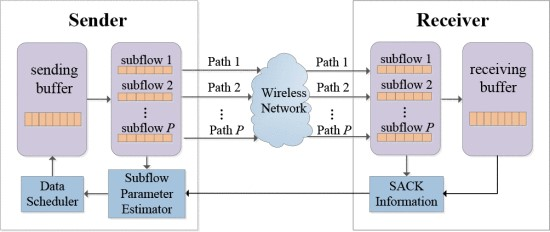
\includegraphics[width=2in]{mptcp_paper/assets/method-model.jpg}
\caption{The model of MPTCP in a heterogeneous wireless network \cite{NewMethod:2018}.}
\label{fig:method-model}
\end{figure}
\subsection{Stage One}
\label{sub:stage-one}
The model consists of a sender, a receiver, and $P$ wireless paths. The sender and receiver have established an MPTCP connection along with $P$ subflows. Suppose that all the subflows are independent, and the characteristics of subflow $i(1 \le i \le P)$ are denoted by the bandwidth $BW_i$, round trip time $RTT_i$ and packet loss rate $PLR_i$, respectively.

In order to adjust packet scheduling based on a subflow’s RTT to minimize out-of-order packet arrival described in Section \ref{sec:mptcp}, a \emph{forward prediction} of the amount of the earlier-arriving packets, denoted as $N_i$, must be estimated. Then subflow $i$ should be allocated from the $(N_{i}+1)-\mathrm{th}$ packet in the sending buffer to keep the packets arriving in order. Figure \ref{fig:subflow_varied} illustrates this concept. Subflow A is the fastest subflow, and no packets will arrive before the packets are delivered on A. Subflow B is slower than A; in this case, two packets will arrive on A before one packet arrives on B. Subflow C is the slowest, and four packets will arrive on A, and two packets arrive on B before one packet is delivered on C.

\begin{figure}
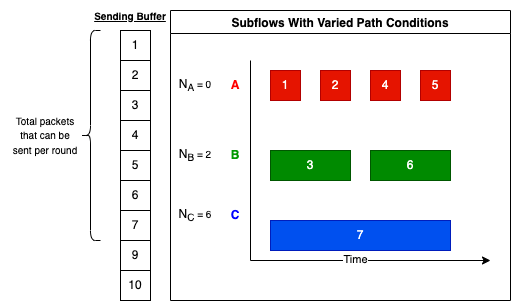
\includegraphics[width=2.5in]{mptcp_paper/assets/subflow_varied.png}
\caption{Illustration of forward prediction. Note that each rectangle represents a single packet of the same data-width-- a thinner retangle means it took less time to send the packet}
\label{fig:subflow_varied}
\end{figure}

$T_i$ represents the duration of the packet sent from the sender to the receiver in subflow $i$. Then $T_i$ can be directly set as $RTT_i/2$, the authors assume the path conditions to be the same in both directions of the subflow in this calculation. During the time of $T_i$, the amount of data sent through another faster subflow $j(RTT_j<RTT_i)$, denoted as $DATA_{i,j}$, can be calculated by:
\begin{equation*} 
DATA_{i,j}=BW_{j}\cdot T_{i}\cdot(1-PLR_{j})=BW_{j}\cdot\frac{RTT_{i}}{2}\cdot(1-PLR_{j})
    \tag{1}
    \label{eq:stage-one-1}
\end{equation*}
where $(1 \le i \le P)$ and $RTT_j<RTT_i$.

Then the amount of data sent simultaneously through all the other subflows with smaller $RTT$ than subflow $j$ during the time of $T_i$, denoted as $DATA_i$, is calculated by

\begin{equation*} 
\label{eq:stage-one-2} \\
\resizebox{1\hsize}{!}{DATA_{i}=\sum_{\mathop{1\leq j\leq P}_{RTT_{j} < RTT_{i}}} DATA_{i,j}= \sum_{\mathop{1\leq j\leq P}_{RTT_{j} < RTT_{i}}} BW_{j}\cdot\frac{RTT_{i}}{2}\cdot(1-PLR_{j})} \tag{2} 
\end{equation*}

Next, the authors suppose each packet has a fixed packet length maximum segment size (MSS) of TCP packet. The value of $N_i$ is evaluated as

\begin{equation*} 
    N_{i}=\left\lfloor\frac{DATA_{i}}{MSS}\right\rfloor 
    \tag{3}
    \label{eq:stage-one-3}
\end{equation*}
where $\left\lfloor x\right\rfloor$ denotes the largest integer less than or equal to $x$

As data is transmitted, a simple exponential smoothing statistical method is used to periodically estimate all the path characteristics such as bandwidth, RTT, and packet loss rate.  For subflow $i$, the value of $RTT_i$ is updated per round of transmission. $SRTT_i$ is the smoothed $RTT_i$. More recent observations better reflect the current state of a path, therefore the $\alpha$ smoothing parameter is set to a value between 0.8 and 0.9 in order to weigh the most recent observations more heavily in the prediction.
\begin{equation*} 
    SRTT_{i}=\alpha\cdot SRTT_{i}+(1-\alpha)\cdot RTT_{i} 
    \tag{4}
    \label{eq:srtt}
\end{equation*}

Bandwidth $BW_i$ and the packet loss rate $PLR_i$ for subflow $i$ can be calculated by

\begin{align*} BW_{i}&=\frac{send_{i}\cdot MSS}{t_{i}} \tag{5}\label{eq:bandwidth} \\
\qquad PLR_{i}&=\frac{loss_{i}}{send_{i}} \label{eq:packet-lose-rate}\tag{6} \end{align*}
where $t_i$ is the estimation period, which the authors set as $5*RTT_i$ to guarantee the statistical characteristic. $send_i$ and $loss_i$ represent the transmitted and lost packets during time period $t_i$.  This allows $BW_i$ and $PLR_i$ to be estimated using the same weighted average form of simple exponential smoothing as $SRTT_i$ where $SBW_i$ is the smoothed $BW_i$ and $SPLR_i$ is the smoothed $PLR_i$. Both $\beta$ and $\gamma$ are smoothing parameters and weigh smoothing with the same values as $\alpha$
\begin{align*}  SBW_{i}&=\beta\cdot SBW_{i}+(1-\beta)\cdot BW_{i}, \label{eq:sbw} \tag{7}\\ SPLR_{i}&=\gamma\cdot SPLR_{i}+(1-\gamma)\cdot PLR_{i}, \label{eq:splr} \tag{8} \end{align*}

\subsection{Stage Two}

Recall that $N$ is the predicted number of packets that can be transmitted simultaneously through all the faster paths. The estimation of the scheduling value $N$ may not be precise in a real heterogeneous wireless environment because, in stage one, the authors assume a path is stable over a short period of time. In a case where the path condition changes quickly, the prediction error will accumulate rapidly. In this stage, the authors adjust the scheduling value to minimize deviations between the predicted and the actual values. To do this, the authors rely on an additional TCP option called selective acknowledgment (SACK). The information provided by SACK allows the receiver to describe which pieces of data it has received from the sender. This enables the sender to re-transmit only the missing data needed by the receiver \cite{Stevens:2011}. Denote $\delta_{i}(n)$ as the adjustment value of subflow $i$ in the $n-\mathrm{th}$ round, after computing the scheduling value $N_{i}(n)$ at the start of the $n-\mathrm{th}$ round, $N_{i}(n)$ should be adjusted by
\begin{equation*} N_{i}^{\prime}(n)=N_{i}(n)+\delta_{i}(n) \label{eq:adjustment} \tag{9} \end{equation*}
where $N_{i}^{\prime}(n)$ is the modified estimation value and will be used for the scheduling of subflow $i$ in the  $n-\mathrm{th}$ round. The adjustment $\delta_{i}(n)$ is dynamically updated by
\begin{equation*} \delta_{i}(n+1)=\lfloor\delta_{i}(n)+\theta\cdot\sigma_{i}(n)\rfloor  \label{eq:adjustment-update} \tag{10} \end{equation*}
where $\delta_{i}(n+1)$ is the updated adjustment value for the next round, $\theta$ is the updating parameter which is set as 1/8, so the integer truncation of $\lfloor\cdot \rfloor$ is needed. The deviation value obtained at the end of the $n^{th}$ round, $\sigma_i(n)$, is based on the feedback information provided by SACK, which indicates the data that was not received by the sender during the transmission round. The authors consider two cases, one in which the estimation of the scheduling value $N_{i}(n)$ is greater than the actual value and one in which the estimation value is less than the actual value.

\subsubsection{Case One}

Consider $N_{i}(n)$ is greater than the actual value, which means more packets are scheduled for transmission on the faster subflows than are actually sent.  This means that subflow $i$ is behaving \emph{faster} than expected (either because subflow $i$ has sped up, or because the previously faster subflows have slowed down). The sequence numbers, including both the data sequence number and subflow sequence number, of the missing packets in the receiver's buffer are recorded in the corresponding SACKs and returned to the sender. The sender can utilize the receiver’s SACK information to determine if the sender is missing data transmitted on another subflow. Missing packets, or holes, indicate to the scheduler that data is arriving faster on subflow $i$ and the predicted scheduling value should be decreased. $h_{i,k}(n)$ represents the number of holes belonging to the faster subflow k in the $n-\mathrm{th}$ round, then the deviation value $\sigma_{i}(n)$ should be updated as

\begin{equation} 
\sigma_{i}(n)\leftarrow\sigma_{i}(n)- \sum_{\substack{1\leq k\leq P \\ RTT_{k} < RTT_{i}}}h_{i,k}(n)  
\label{eq:case-one} 
\tag{11} 
\end{equation}

\subsubsection{Case Two}

Consider $N_{i}(n)$ is less than the actual value, which indicates fewer packets are scheduled for the faster subflows during the scheduling time of subflow $i$. For a faster subflow $j$, after transmitting the scheduled packets, the proposed scheduling method will continually send new packets with more data, meaning larger data sequence number DSNs, which may arrive earlier than the packets transmitted from slower subflow $i$. The sender may receive the SACK from subflow $j$, which indicates that there are holes in the DSNs, but the SSNs of subflow $j$ are successive, indicating that the missing packets are caused by inappropriate scheduling for the subflows slower than it and the predicted scheduling value should be increased.
\begin{equation} 
\sigma_{i}(n)\leftarrow\sigma_{i}(n)+ \sum_{\substack{1\leq k\leq P \\ RTT_{m} < RTT_{i}}}h_{i,m}(n) 
\label{eq:case-two} \tag{12} 
\end{equation}
In summary, when a transmission round begins, the algorithm \ref{alg:scheduling-method} estimates a scheduling value for each subflow. Then the algorithm modifies the scheduling value with the adjustment value. At the end of the round, the sender recalculates the path characteristics for the next scheduling and computes the deviation value of the prediction based on the TCP SACK information from the receiver. The adjustment value is also updated with the deviation for the next round. In addition, the authors calculated computation complexity of dynamic packet scheduling algorithm to be linear $O(n)$, which means that the run-time of the algorithm grows almost linearly with the input size.
\begin{algorithm}[H]
\caption{Dynamic Packet Scheduling Method \cite{NewMethod:2018}.}
\begin{algorithmic}[1]
\State{Sender starts the n-th round transmission of subflow $i$,
estimates the scheduling value $N_i(n)$ according to (\ref{eq:stage-one-1},~\ref{eq:stage-one-2},~\ref{eq:stage-one-3});}
\State{ Modify $N_i(n)$ with the adjustment value $\delta_{i}(n)$ by \eqref{eq:adjustment};}
\State{Subflow $i$ sends from the $(N_i(n)+1)$-th packet in buffer;}
\State{Update the path characteristics $RTT_i$, $BW_i$ and $PLR_i$;}
\State{Sender receives the SACK of subflow $i$ and there is no
missing packet of subflow $i$ itself}
    \If{some holes in DSNs belong to the faster subflows,
decrease the deviation value $\sigma_{i}(n)$ by \eqref{eq:case-one};}
    \EndIf
    \If{some holes in DSNs belong to the slower subflows,
increase the deviation value $\sigma_{i}(n)$ by \eqref{eq:case-two};}
    \EndIf

\State{Update the updated adjustment value $\delta_{i}(n+1)$ for the next
round with $\sigma_{i}(n)$ by \eqref{eq:adjustment-update}}
\end{algorithmic}
\label{alg:scheduling-method}
\end{algorithm}

\section{Results}
\label{sec:results}

The authors used the \emph{ns-3} network simulator software (see \cite{NewMethod:2018} for details) to evaluate the performance of the proposed packet scheduling method in Section \ref{sec:method}. The proposed method was compared with two other packet scheduling schemes, \emph{Forward Prediction Scheduling} (FPS) and \emph{Dynamic Packet Scheduling and Adjusting with Feedback} (DPSAF). FPS uses the forward prediction method to estimate a scheduling value but ignores the packet loss rate and bandwidth. DPSAF considers the packet loss rate and also uses the TCP SACK information as feedback to adjust the scheduling value. However, DPSAF does not take the path bandwidth into consideration and uses a more complicated analysis model with a high computation complexity.

The network topology of the simulation is described in Figure \ref{fig:ns3-model}. The client establishes three MPTCP subflows \emph{A}, \emph{B}, and \emph{C} with the server. Each subflow path consists of wired and wireless links with varying path characteristics. In the simulation, the authors manipulated the packet loss rate from 0.1\% to 3\% and the receiving buffer size from 16KB to 512KB on subflow \emph{C} to compare the performance of the packet scheduling methods.
\begin{figure}
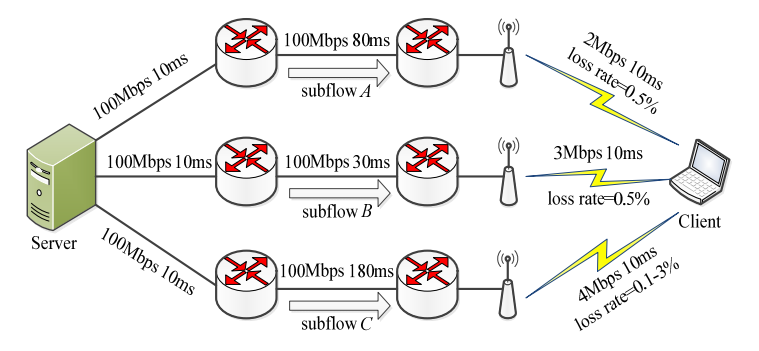
\includegraphics[width=2.5in]{mptcp_paper/assets/ns3-model.png}
\caption{Simulation topology of MPTCP used for scheduling method comparison \cite{NewMethod:2018}.}
\label{fig:ns3-model}
\end{figure}
\subsection{Increase In Packet Loss Rate}
\label{sub:increase-plr}
In the first simulation, the packet loss rate of subflow \emph{C} is increased from 0.1\% to 3\%. Figure \ref{fig:plr-increased} shows that the throughput performance is degraded across all scheduling methods as packet loss rate increases. The FPS scheduling method performs the worst as it only considers the path latency. The deviation in the FPS scheduling value increases with increased packet loss and is not adjusted to account for packet loss increase. The newly proposed method slightly outperforms DPSAF by taking the path bandwidth into consideration, which helps to enhance the scheduling value accuracy and the overall throughput.

In addition to throughput, the average number of out-of-order packets in the receiving buffer was also measured as packet loss increased on subflow \emph{C}. Fewer out-of-order packets indicate a more favorable result. Figure \ref{fig:plr-increased} shows that as packet loss increases, the average out-of-order packets increase across all scheduling methods. However, the proposed scheduling method outperforms both FPS and DPSAF, consistently having the lowest average out-of-order packets as packet loss increases.
\begin{figure}
\centering
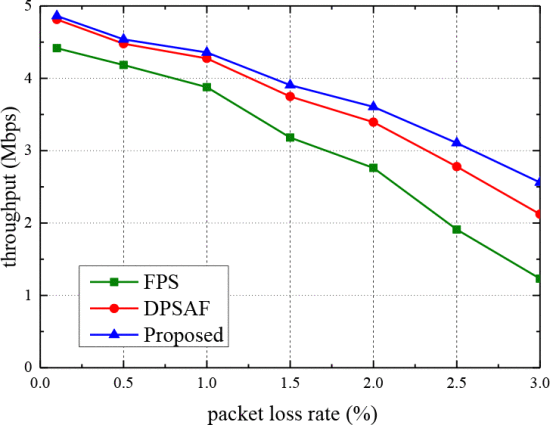
\includegraphics[width=1.5in]{mptcp_paper/assets/packet-loss.png}
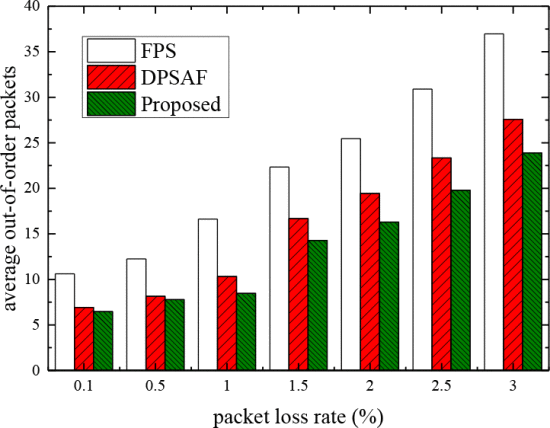
\includegraphics[width=1.5in]{mptcp_paper/assets/out-of-order-plr.png}
\caption{Throughput and average out-of-order packets as packet loss rate increases \cite{NewMethod:2018}.} 
\label{fig:plr-increased}
\end{figure}

In the next simulation, the MPTCP receiving buffer size was varied from 16 KB to 512 KB, and packet loss rate of subflow \emph{C} was held constant at 1\%. The overall throughput of the three scheduling methods increased as buffer size increased. The overall performance increase occurs because when the buffer size is large enough, out-of-order packets can be temporarily stored and do not block the transmission of additional packets. Figure \ref{fig:buffer-size-increase} shows that the proposed scheduling method outperformed both FPS and DPSAF. However, as buffer size increased beyond 128KB the proposed method only slightly outperformed DPSAF in overall throughput.

Figure \ref{fig:buffer-size-increase} shows the average out-of-order packets as the size of the receiving buffer increased. As the receiving buffer becomes larger, more packets can be stored in the buffer which leads to an increase in the number of out-of-order packets, as higher sequence number packets are not blocked from being received. As the buffer size increased, all three scheduling methods had an increase in the total number of out-of-order packets. The proposed scheduling method has the lowest average out-of-order packets compared to FPS and DPSAF across all tested buffer sizes.
\begin{figure}
\centering
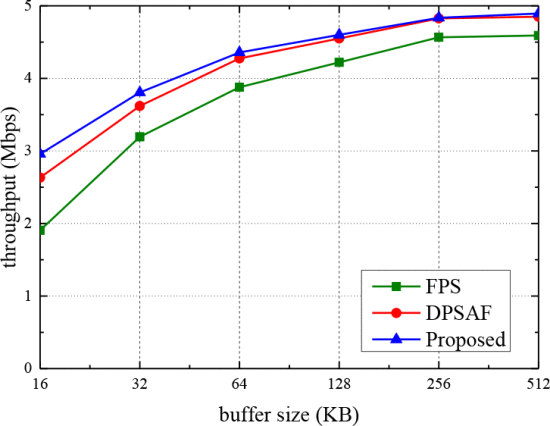
\includegraphics[width=1.5in]{mptcp_paper/assets/throughput.png}
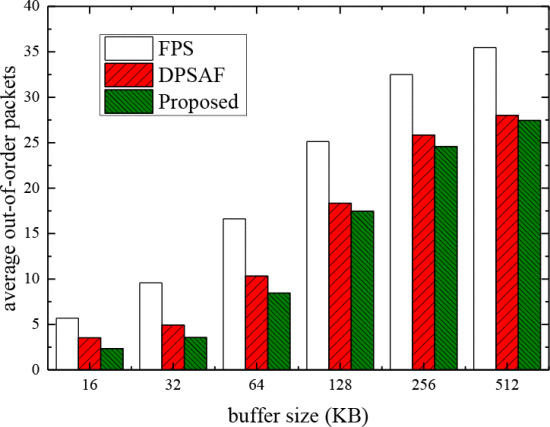
\includegraphics[width=1.5in]{mptcp_paper/assets/buffer-size.png}
\caption{Throughput and average out-of-order packets as buffer size increases \cite{NewMethod:2018}}
\label{fig:buffer-size-increase}
\end{figure}

\section{Conclusion}
\label{sec:conclusion}

MPTCP is an exciting addition to the existing network infrastructure currently in place around the world. The backward compatibility MPTCP has with TCP means that MPTCP is likely to be widely adopted across the network industry to improve connection quality. While MPTCP presents new challenges related to packet scheduling across subflows, new techniques are being developed to minimize MPTCP packet scheduling issues. The method described in this paper demonstrates throughput performance improvement and a reduction in the number of out-of-order packets by considering network metrics not used in current MPTCP scheduling method implementations.

%%
%% The acknowledgments section is defined using the "acks" environment
%% (and NOT an unnumbered section). This ensures the proper
%% identification of the section in the article metadata, and the
%% consistent spelling of the heading.
\begin{acks}
I would like to thank my advisor Peter Dolan, Ph.D. for providing outstanding feedback and guidance throughout the research and writing of this paper. I also want to thank Kristin Lamberty, Ph.D for facilitating the senior seminar process and Kevin Arhelger for his professional review and feedback.
\end{acks}

\bibliographystyle{ACM-Reference-Format}
\bibliography{mptcp_paper}
\end{document}
\endinput
%%
%% End of file `sample-sigplan.tex'.